\chapter*{Appendix - Test Automation Pyramid}

\label{testing-pyramid}

The test automation pyramid is a metaphor intended to encourage teams to use small, fast, isolated tests as the foundation of their test automation strategy. The more of the application a test exercises, the fewer of these tests we want in our automated test suite.

\begin{center}
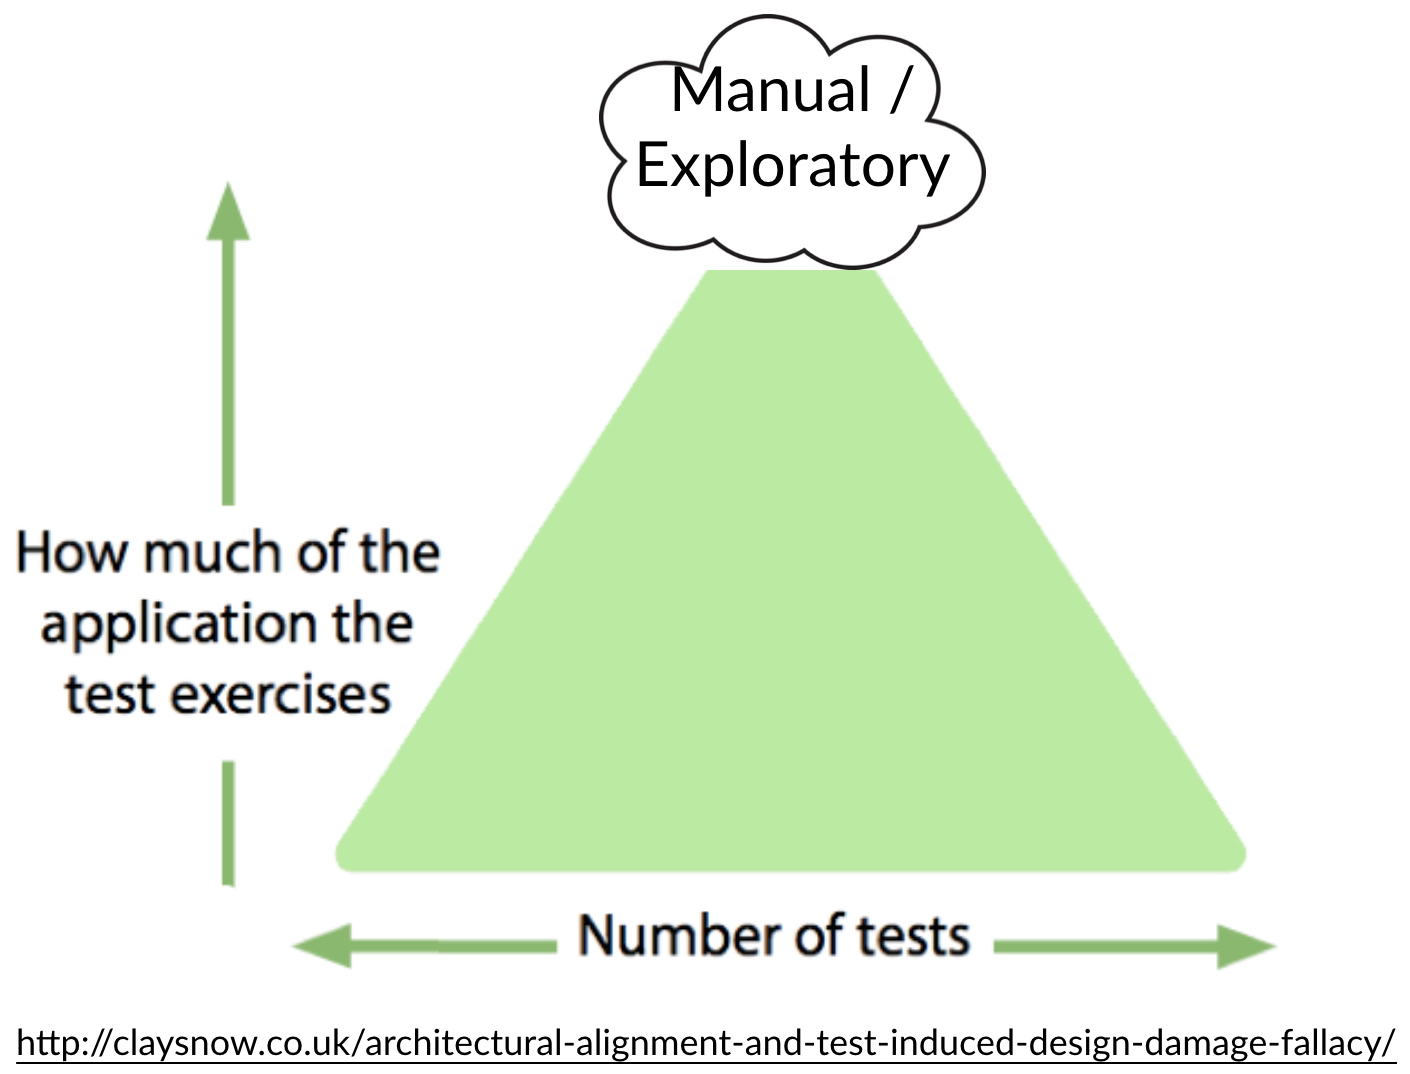
\includegraphics[height=10cm]{images/testing-pyramid}
\end{center}

\section*{The purpose of a test}

Every test should have a reason for existing. The test automation pyramid is often drawn divided into 3 sections: bottom, middle and top.

\begin{itemize}
    \item \emph{Bottom}: small, fast, isolated tests that verify that the developer wrote the code they intended to.
    \item \emph{Middle}: tests that verify the interaction between a few components of the system - these tests are intended to check the protocols, messages and error handling which define how the system should behave
    \item \emph{Top}: tests that verify that the whole system "hangs together" - these can be thought of as smoke tests that check the deployment of the system to an environment
    \begin{itemize}
        \item Have we got the right database connection credentials? 
        \item Are we hitting the right service endpoints?
        \item Can we access some representative user journeys?
    \end{itemize}
\end{itemize}